\documentclass[12pt]{article}

\usepackage{tikz}
\usepackage{geometry}

\usetikzlibrary{mindmap}

\pagestyle{empty}

\geometry{landscape, margin=1cm}


\begin{document}
\begin{center}
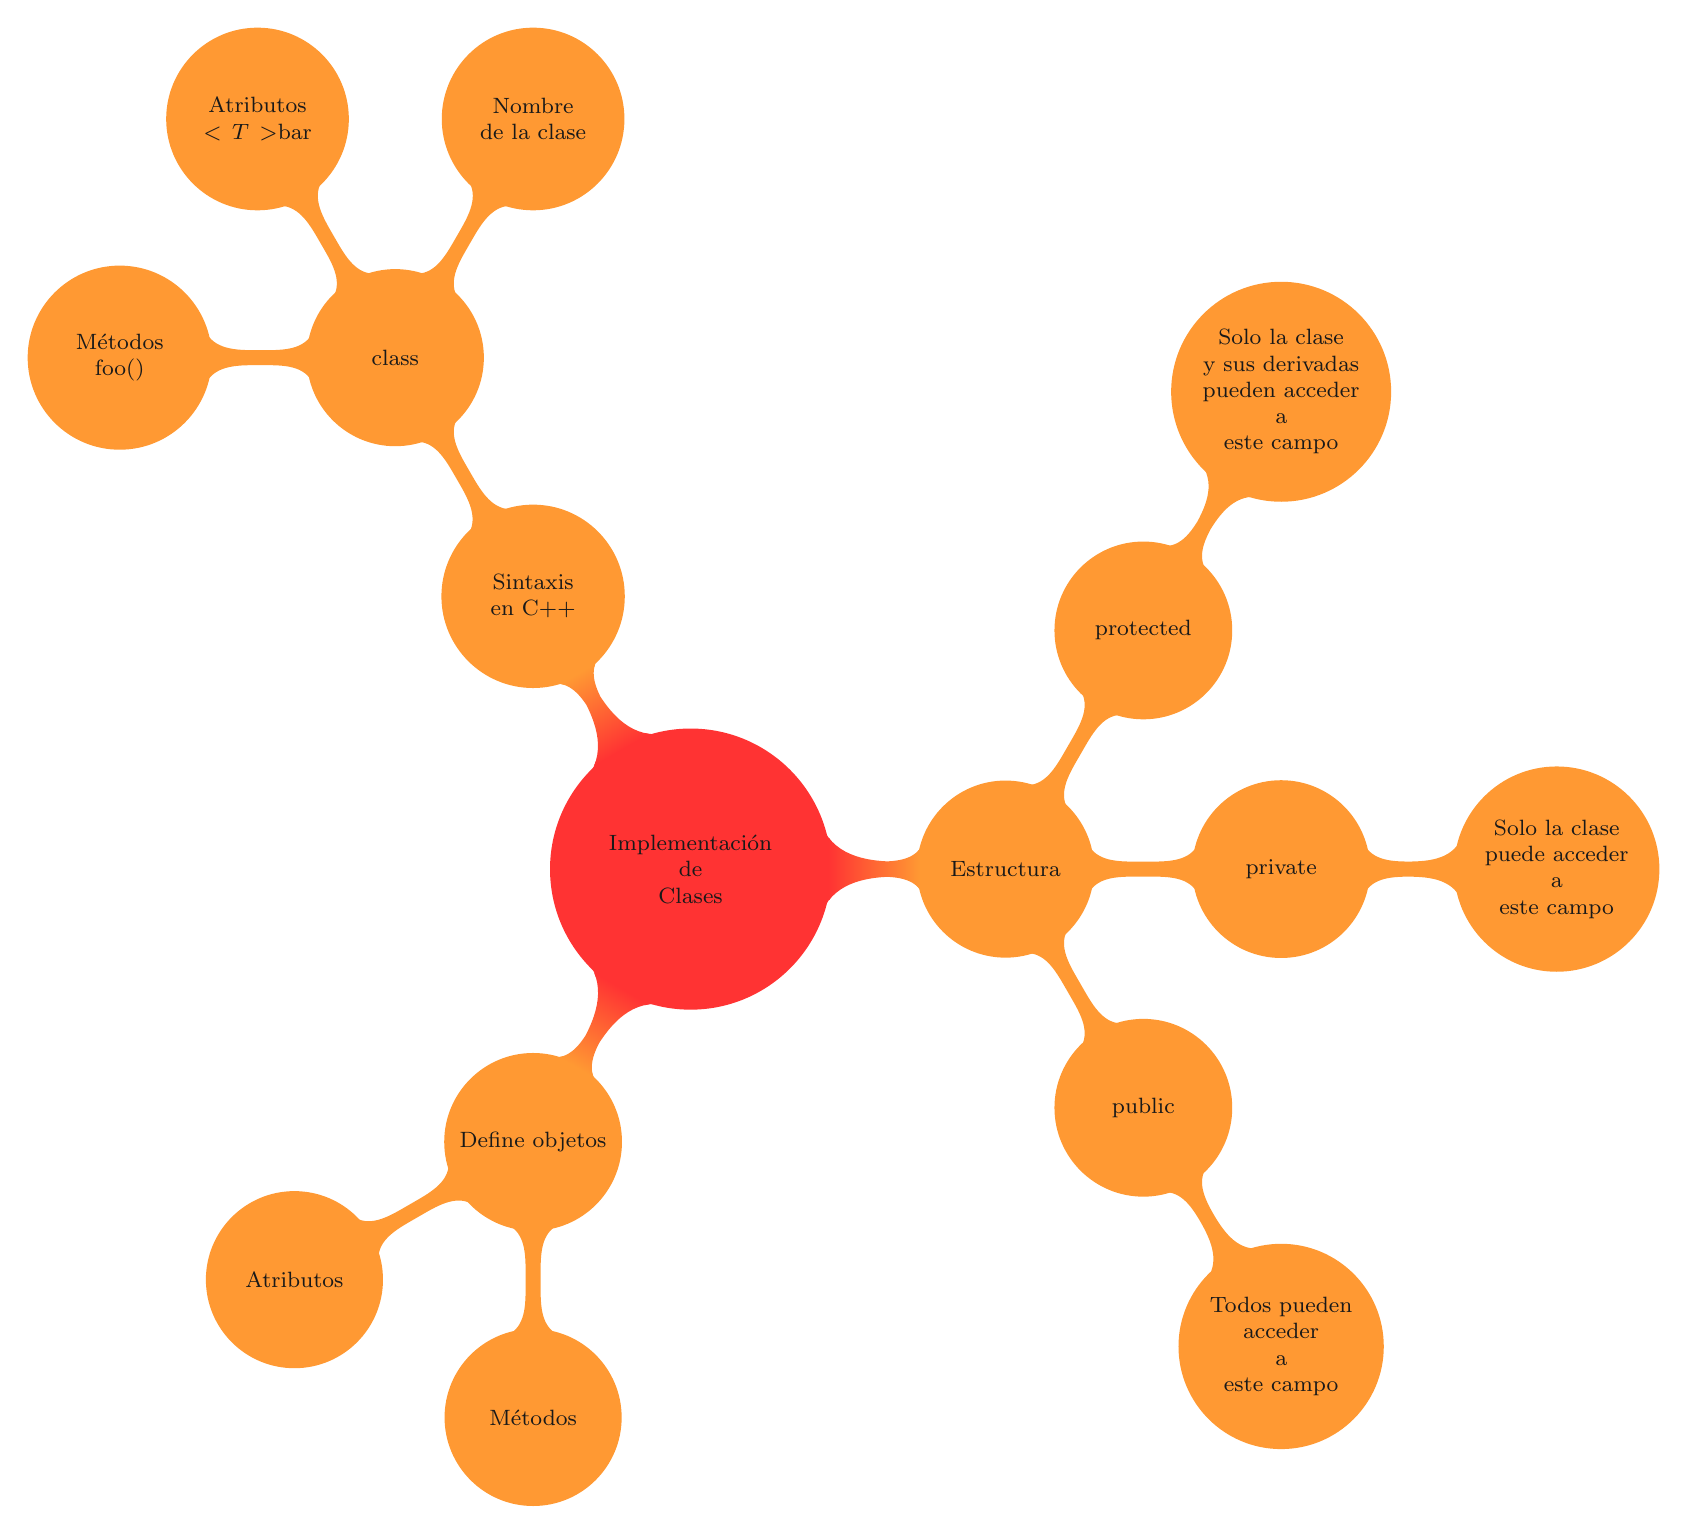
\begin{tikzpicture}[small mindmap, grow cyclic, every node/.style=concept, concept color=red!80, text=black!90, minimum size=3.5cm,
    level 1/.style={level distance=4.5cm,sibling angle=360/3},
    level 1/.style={level distance=4.0cm,sibling angle=360/3},
    level 2/.style={level distance=3.5cm,sibling angle=60},
    level 3/.style={level distance=3.5cm,sibling angle=60},
    ]

    \node{Implementación\\de\\Clases}
    child[concept color=orange!80, minimum size=2cm] { node {Define objetos}
        child { node {Atributos} }
        child { node {Métodos} }
    }
    child[concept color=orange!80, minimum size=2cm] { node {Estructura}
        child { node {public}
            child { node {Todos pueden acceder\\a\\este campo} }
        }
        child { node {private}
            child { node {Solo la clase\\puede acceder\\a\\este campo} }
        }
        child { node {protected}
            child { node {Solo la clase\\y sus derivadas\\pueden acceder\\a\\este campo} }
        }
    }
    child[concept color=orange!80, minimum size=2cm] { node {Sintaxis en C++}
        child { node {class}
            child { node {Nombre de la clase} }
            child { node {Atributos\\$<T>$bar} }
            child { node {Métodos\\foo()} }
        }
    }
    ;
\end{tikzpicture}
\end{center}
\end{document}
